\pdfvariable minorversion=7
\pdfvariable inclusioncopyfonts=1

\documentclass{arialFHGR} % use either arialFHGR or timesFHGR
\newcommand{\haupttitel}{Titel der Studienarbeit}
\newcommand{\untertitel}{Untertitel}
\newcommand{\zusammenfassung}{Abstract}
\newcommand{\autorenschaft}{Max Mustermann}
\newcommand{\studiengang}{BSc Information Science}
\newcommand{\matrikelnummer}{00-000-000}
\newcommand{\adresse}{Musterstrasse 1}
\newcommand{\ort}{Musterhausen}
\newcommand{\plz}{0000}
\newcommand{\department}{[Departement]}
\newcommand{\institute}{[Institutsname]}
\newcommand{\modul}{WIAGRU}
\newcommand{\email}{max.mustermann@stud.fhgr.ch}
\newcommand{\refe}{Prof. Dr. Eva Mustermann}
\newcommand{\coRefe}{Julian Junke}
\newcommand{\abgabedatum}{01.10.1963}
\newcommand{\abgabedatumRFC}{1963-10-01}
\newcommand{\sprache}{de}
\newcommand{\schlagworte}{Keyword 1, Keyword 2}

\usepackage{setspace, fancyhdr, lscape, floatrow, caption, inputenc, graphicx, enumitem, tabularx, colorprofiles, xstring, hyphenat, chngcntr, xspace, listings, pdfpages}

\usepackage[left=3cm,right=2.5cm,top=2.5cm,bottom=2cm]{geometry}
\usepackage[backend=biber,style=apa,citestyle=apa]{biblatex}
\usepackage[autostyle]{csquotes}
\usepackage[english, nswissgerman]{babel}
\usepackage[titles]{tocloft}
\usepackage[hang,flushmargin]{footmisc}

% Settings for glossary
\usepackage[acronym,toc=true,xindy,nopostdot=true,nonumberlist,nogroupskip=true]{glossaries}
\loadglsentries{content/01_vorspann/01.4_abkuerzungsverzeichnis_glossar}
\setglossarystyle{alttree}
\setglossarypreamble[acronym]{\vspace*{-8pt}}
\makeglossaries
\glsaddall
\glsfindwidesttoplevelname

\graphicspath{{content/00_assets}} % Set path as default for including graphics
\addbibresource{content/00_assets/quellen.bib} % Add bibliography entries

% cite with acronym. 
% Example input: \citeAbbr{schweizerische_archivdirektorinnen-_und_archivdirektorenkonferenz_informations-_2018}{adk}
\newcommand{\parenciteabbr}[2]{(\acrlong{#2} [\acrshort{#2}], \citeyear{#1})}
\newcommand{\textciteabbr}[2]{\acrlong{#2} (\acrshort{#2}, \citeyear{#1})}
\newcommand{\acrfullSqBr}[1]{\acrlong{#1} [\acrshort{#1}]}

\setmonofont{Courier New}

% Settings for listings
\lstdefinestyle{codeStyle}{
    belowcaptionskip=6pt,
    belowskip=3pt,
    breaklines=true,
    numbers=left,
    basicstyle=\footnotesize\ttfamily,
    extendedchars=true,
    frame=single,
    captionpos=t,
    numberbychapter=false,
    xleftmargin=4pt,
    xrightmargin=4pt
}
\lstset{style=codeStyle}

% Settings for blockquote
\SetBlockEnvironment{quotation}
\patchcmd{\quotation}{\rightmargin}{\leftmargin 1.3cm \rightmargin 0}{}{}
\NewCommandCopy{\oldblockquote}{\blockquote}
\renewcommand{\blockquote}[1]{\oldblockquote{\noindent #1}}

% Settings for figure and table
\counterwithout{figure}{chapter}
\counterwithout{table}{chapter}

\floatsetup[figure]{
    capposition=above,
    captionskip=2pt
}

\DeclareCaptionLabelFormat{figTitle}{%
    Abbildung \the\numexpr\value{figure}\relax\\
}

\captionsetup[figure]{
    font={normalsize,stretch=1.0},
    labelfont=bf,
    labelsep=none,
    labelformat=figTitle,
    textfont=it,
    justification=raggedright,
    singlelinecheck=false,
    position=above,
}

\floatsetup[table]{
    capposition=above,
    captionskip=2pt
}

\DeclareCaptionLabelFormat{tabTitle}{%
    Tabelle \the\numexpr\value{table}\relax \\
} 

\captionsetup[table]{
    font={normalsize,stretch=1.0},
    labelfont={bf},
    labelsep=none,
    labelformat=tabTitle,
    textfont=it,
    justification=raggedright,
    singlelinecheck=false,
    position=above
}

\floatsetup[lstlisting]{
    capposition=above,
    captionskip=2pt
}

\DeclareCaptionLabelFormat{codeTitle}{%
    Programmcode \the\numexpr\value{lstlisting}\relax \\
} 

\captionsetup[lstlisting]{
    font={normalsize,stretch=1.0},
    labelfont={bf},
    labelsep=none,
    labelformat=codeTitle,
    textfont=it,
    justification=raggedright,
    singlelinecheck=false,
    position=above
}

\renewcommand{\thetable}{\arabic{table}}
\renewcommand{\thefigure}{\arabic{figure}}

% Einstellungen für tocloft / Settings for tocloft
\renewcommand{\cftfigpresnum}{Abb.~}
\renewcommand{\cfttabpresnum}{Tab.~}
\renewcommand{\cftfigaftersnum}{:}
\renewcommand{\cfttabaftersnum}{:}
\setlength{\cftfignumwidth}{2cm}
\setlength{\cfttabnumwidth}{2cm}
\setlength{\cftfigindent}{0cm}
\setlength{\cfttabindent}{0cm}

\setstretch{1.3} % Zeilenabstand / line spacing
\renewcommand{\arraystretch}{1.3} % Zeilenabstand innerhalb von Tabellen / line spacing in tables
\setlength{\parindent}{1.3cm} % Einzug neuer Absatz / Indentation new paragraph
\fancyhf{}
\renewcommand{\headrulewidth}{0pt}
\pagestyle{fancyplain}
\rfoot{\footnotesize\thepage}

\usepackage[pdfa]{hyperref}
\usepackage{hyperxmp}
\usepackage{embedfile}
\pdfvariable omitcidset=1

% 
\newcommand{\chapterNoNr}[1]{%
    \chapter*{#1}
    \addcontentsline{toc}{chapter}{#1} %
}%

\newcommand{\note}[1]{%
    \doublespacing\raggedright\footnotesize{\textit{Anmerkung:} #1}
}%

\newcommand{\sic}{%
    [\textit{sic}]\xspace
}%

\makeatletter
\def\l@lstlisting#1#2{\@dottedtocline{1}{0em}{2em}{Programmcode #1}{#2}}
\makeatother

\hypersetup{%
    pdflang=\sprache,
    pdftitle={\haupttitel},
    pdfsubtitle={\untertitel},
    pdfauthor={\autorenschaft},
    pdfdate={\abgabedatumRFC},
    pdfsubject={\zusammenfassung},
    pdfkeywords={\modul, \schlagworte},
    pdfcontactaddress={\adresse},
    pdfcontactcity={\ort},
    pdfcontactpostcode={\plz},
    pdfcontactemail={\email},
    colorlinks,
    unicode,
    allcolors=black,
    pdfapart=2,
    pdfaconformance=U
}

% 
\immediate\pdfobj stream attr{/N 3} file{sRGB.icc}
\pdfcatalog{%
  /OutputIntents [
    <<
      /Type /OutputIntent
      /S /GTS_PDFA1
      /DestOutputProfile \the\pdflastobj\space 0 R
      /OutputConditionIdentifier (sRGB)
      /Info (sRGB)
    >>
  ]
}

\begin{document}

    \renewcommand{\contentsname}{Inhaltsverzeichnis}
    \renewcommand{\listfigurename}{Abbildungsverzeichnis}
    \renewcommand{\listtablename}{Tabellenverzeichnis}
    \renewcommand{\acronymname}{Abkürzungsverzeichnis}
    \renewcommand{\lstlistlistingname}{\texorpdfstring{Programmcodeverzeichnis\bigskip}{Programmcodeverzeichnis}}
    
    % Start Vorspann
    
    \pagenumbering{Roman} % Begin roman pagenumbering

    % Titelblatt für eine Studienarbeit
     \begin{titlepage}
    
    \begin{center}
        Fachhochschule Graubünden, \institute \\
        \vspace{30mm}
        \huge\textbf{\haupttitel}\\
        \hfill \break
        \large{(\untertitel)}
    \end{center}
    
    \vfill
    
    \begin{flushleft}
    Name: \autorenschaft\\
    Studiengang: \studiengang\\
    Matrikelnr.: \matrikelnummer\\
    Adresse: \adresse, \plz~\ort\\
    E-Mail: \email\\
    ~\\
    Modul: \modul\\
    Referent/in: \refe\\
    Koreferent/in: \coRefe\\
    ~\\
    Abgabedatum: \abgabedatum
    \end{flushleft}
    
    \vspace{20mm}
    
\end{titlepage}

    % ODER für eine Abschlussarbeit
    % \begin{titlepage}
    \begin{center}
        {\large
            {\Large\textbf{\haupttitel}} \\
            \textit{\untertitel} \\
            ~\\
            An der Fachhochschule Graubünden \\
            \department \\
            \institute \\
            \vspace{2mm}
            im Studiengang \studiengang{} eingereichte \\
            ~\\
            {\Huge\textbf{Bachelorarbeit}} \\
            ~\\
            zur Erlangung des akademischen Grades \\
            eines Bachelor of Science (B.Sc.)
    
            \vspace{40mm}
            vorgelegt von \\
            \vspace{4mm}
            {\Large\textbf{\autorenschaft}} \\
            \vspace{4mm}
            Matrikelnr.: \matrikelnummer \\
            E-Mail: \email \\
            ~\\~\\
            Erstgutachter/in: \refe \\
            Zweitgutachter/in: \coRefe \\
            ~\\
            Eingereicht am: \abgabedatum
        } % end large
    \end{center}
\end{titlepage}


    \chapter*{Abstract}
Sit amet mattis vulputate enim nulla aliquet. Risus at ultrices mi tempus imperdiet nulla malesuada pellentesque. Turpis nunc eget lorem dolor sed viverra ipsum nunc aliquet. Turpis egestas integer eget aliquet nibh praesent. Sed euismod nisi porta lorem mollis aliquam ut porttitor leo. Sem viverra aliquet eget sit. Id leo in vitae turpis massa sed elementum tempus egestas. Pharetra vel turpis nunc eget lorem dolor sed viverra ipsum. Velit ut tortor pretium viverra suspendisse potenti nullam ac. Eget sit amet tellus cras adipiscing enim eu turpis. Pulvinar neque laoreet suspendisse interdum consectetur libero. Consequat interdum varius sit amet mattis vulputate enim nulla aliquet. Amet purus gravida quis blandit turpis cursus in hac habitasse. In aliquam sem fringilla ut morbi tincidunt augue. Tellus molestie nunc non blandit massa enim nec. Mi eget mauris pharetra et ultrices neque.

    \chapter*{Vorwort}
Sit amet mattis vulputate enim nulla aliquet. Risus at ultrices mi tempus imperdiet nulla malesuada pellentesque. Turpis nunc eget lorem dolor sed viverra ipsum nunc aliquet. Turpis egestas integer eget aliquet nibh praesent. Sed euismod nisi porta lorem mollis aliquam ut porttitor leo. Sem viverra aliquet eget sit. Id leo in vitae turpis massa sed elementum tempus egestas. Pharetra vel turpis nunc eget lorem dolor sed viverra ipsum. Velit ut tortor pretium viverra suspendisse potenti nullam ac. Eget sit amet tellus cras adipiscing enim eu turpis. Pulvinar neque laoreet suspendisse interdum consectetur libero. Consequat interdum varius sit amet mattis vulputate enim nulla aliquet. Amet purus gravida quis blandit turpis cursus in hac habitasse. In aliquam sem fringilla ut morbi tincidunt augue. Tellus molestie nunc non blandit massa enim nec. Mi eget mauris pharetra et ultrices neque.

Sit amet mattis vulputate enim nulla aliquet. Risus at ultrices mi tempus imperdiet nulla malesuada pellentesque. Turpis nunc eget lorem dolor sed viverra ipsum nunc aliquet. Turpis egestas integer eget aliquet nibh praesent. Sed euismod nisi porta lorem mollis aliquam ut porttitor leo. Sem viverra aliquet eget sit. Id leo in vitae turpis massa sed elementum tempus egestas. Pharetra vel turpis nunc eget lorem dolor sed viverra ipsum. Velit ut tortor pretium viverra suspendisse potenti nullam ac. Eget sit amet tellus cras adipiscing enim eu turpis. Pulvinar neque laoreet suspendisse interdum consectetur libero. Consequat interdum varius sit amet mattis vulputate enim nulla aliquet. Amet purus gravida quis blandit turpis cursus in hac habitasse. In aliquam sem fringilla ut morbi tincidunt augue. Tellus molestie nunc non blandit massa enim nec. Mi eget mauris pharetra et ultrices neque.

    \tableofcontents % Inhaltsverzeichnis
        
    % List of figures
    \cleardoublepage
    \phantomsection
    \addcontentsline{toc}{chapter}{\listfigurename}
    \listoffigures
    
    % List of tables
    \cleardoublepage
    \phantomsection
    \addcontentsline{toc}{chapter}{\listtablename}
    \listoftables

    % List of acronyms
    \printglossary[type=\acronymtype]

    % List of code
    \cleardoublepage
    \phantomsection
    \addcontentsline{toc}{chapter}{\lstlistlistingname}
    \lstlistoflistings
    \newpage
    % Ende Vorspann
    
    % Start Textteil
    \pagenumbering{arabic} % Begin arabic pagenumbering
    \chapter{Einleitung}
Das ist die Einleitung. Interssantes findest du aber eher im Kapitel \ref{kap:eins}.
    \chapter{Erstes Kapitel}
\label{kap:eins}
Dies ist eine Vorlage für wissenschaftliche Arbeiten an der FHGR nach \textcite{stepanenko_leitfaden_2023}\footnote{Quelle aus dem Intranet (nicht öffentlich zugänglich) von FHGR}. Nachfolgend einige Tipps und Funktionen, welche in der Vorlage enthalten sind.

\section{Glossar und Abkürzungen}
Mit den Befehlen \lstinline|acrlong{zb}|, \lstinline|acrshort{zb}| oder \lstinline|acrfull{zb}| ist das Ausgeben der im Dokument \lstinline{content/00_assets/01_Vorspann/01.4_abkuerzungsverzeichnis_glossar.tex} Einträgen möglich: \acrshort{zb}, \acrshort{zb}, \acrfull{zb}.

\section{Zitieren}
Für das Setzen von Anführungszeichen stehen verschiedene Möglichkeiten zur Verfügung. Mittels \lstinline|\enquote{...}| können Texte in Anführungszeichen gesetzt werden. Zum Beispiel: \\\lstinline|\enquote{Ein wörtliches Zitat}| ergibt \enquote{Das ist ein wörtliches Zitat}. Guillemets können auch mittels \lstinline{"<} und \lstinline{">} gesetzt werden. Als Beispiel \lstinline{"<Ein wörtliches Zitat">} ergibt "<Ein wörtliches Zitat">. Ein Blockzitat kann mittels des Befehls \lstinline|\blockquote{...}| erstellt werden. Die Ausgabe eines Blockzitats sieht folgendermassen aus:

\blockquote{Blockzitate sind wörtliche Zitate von 40 Wörtern oder mehr; sie werden als eigener Absatz ohne Anführungszeichen angeführt. Ein Blockzitat beginnt stets in einer neuen Zeile, wird zur Gänze (also jede Zeile) 1,3 cm oder fünf Leerschritte eingerückt und mit zweizeiligem Abstand geschrieben. Absätze innerhalb eines Blockzitates werden vom neuen Rand des Blockzitates eingerückt. \par Blockzitate werden nicht in Anführungszeichen gesetzt, darin aufscheinende Zitate werden in doppelten Anführungszeichen wiedergegeben. \par Die Quellenangabe am Ende eines Blockzitates steht nach dem letzten schlie"senden Punkt des Zitates in Klammern gesetzt, danach folgt kein weiterer Punkt.\\
\parencite[S. 111]{psychologie_richtlinien_2016}}
\noindent
Weitere Möglichkeiten können der Dokumentation\footnote{http://mirrors.ctan.org/macros/latex/contrib/csquotes/csquotes.pdf} zum \texttt{csquotes} Paket entnommen werden.
\newpage
Für die Quellverwaltung wird das Paket \texttt{biblatex} mit dem APA Zitationsstil verwendet. Die umfangreiche Dokumentation\footnote{https://mirror.metanet.ch/tex-archive/info/translations/biblatex/de/biblatex-de-Benutzerhandbuch.pdf} bietet einen Überblick aller möglichen Befehle. Voraussetzung ist, dass die Quellen erst im BibLaTeX Format unter \lstinline{content/00_assets/quellen.bib} abgelegt sind (z. B. via Zotero / Mendely\footnote{https://www.overleaf.com/learn/how-to/How\_to\_link\_your\_Overleaf\_account\_to\_Mendeley\_and\_Zotero} oder als Datei). Nachfolgend einige Beispiele mit den üblichsten Befehlen:\\
\\
\lstinline|\textcite{diani_black_2016}| gibt als Ausgabe:
\textcite{diani_black_2016}\\
\lstinline|\parencite{diani_black_2016}| gibt als Ausgabe:
\parencite{diani_black_2016}\\
\lstinline|\parencites[S. 10]{diani_black_2016}[S. 20]{stepanenko_leitfaden_2023}| gibt als Ausgabe:
\parencites[S. 10]{diani_black_2016}[S. 20]{stepanenko_leitfaden_2023}\\
\\
Zusätzlich stehen die folgenden eigens im Template definierten Befehle zur Verfügung, bei welchen die im \lstinline{content/01_vorspann/01.4_abkuerzungsverzeichnis_glossar.tex} definierten Abkürzungen verwendet werden können:\\
\\
\lstinline|parenciteabbr{org_2022}{orln}| gibt als Ausgabe: \parenciteabbr{org_2022}{orln}\\
\\
\lstinline|textciteabbr{org_2022}{orln}| gibt als Ausgabe: 
\textciteabbr{org_2022}{orln}\\

\chapter{Ein Bild}
\begin{figure}[H]
    \caption{Überschrift Abbildung 1}
    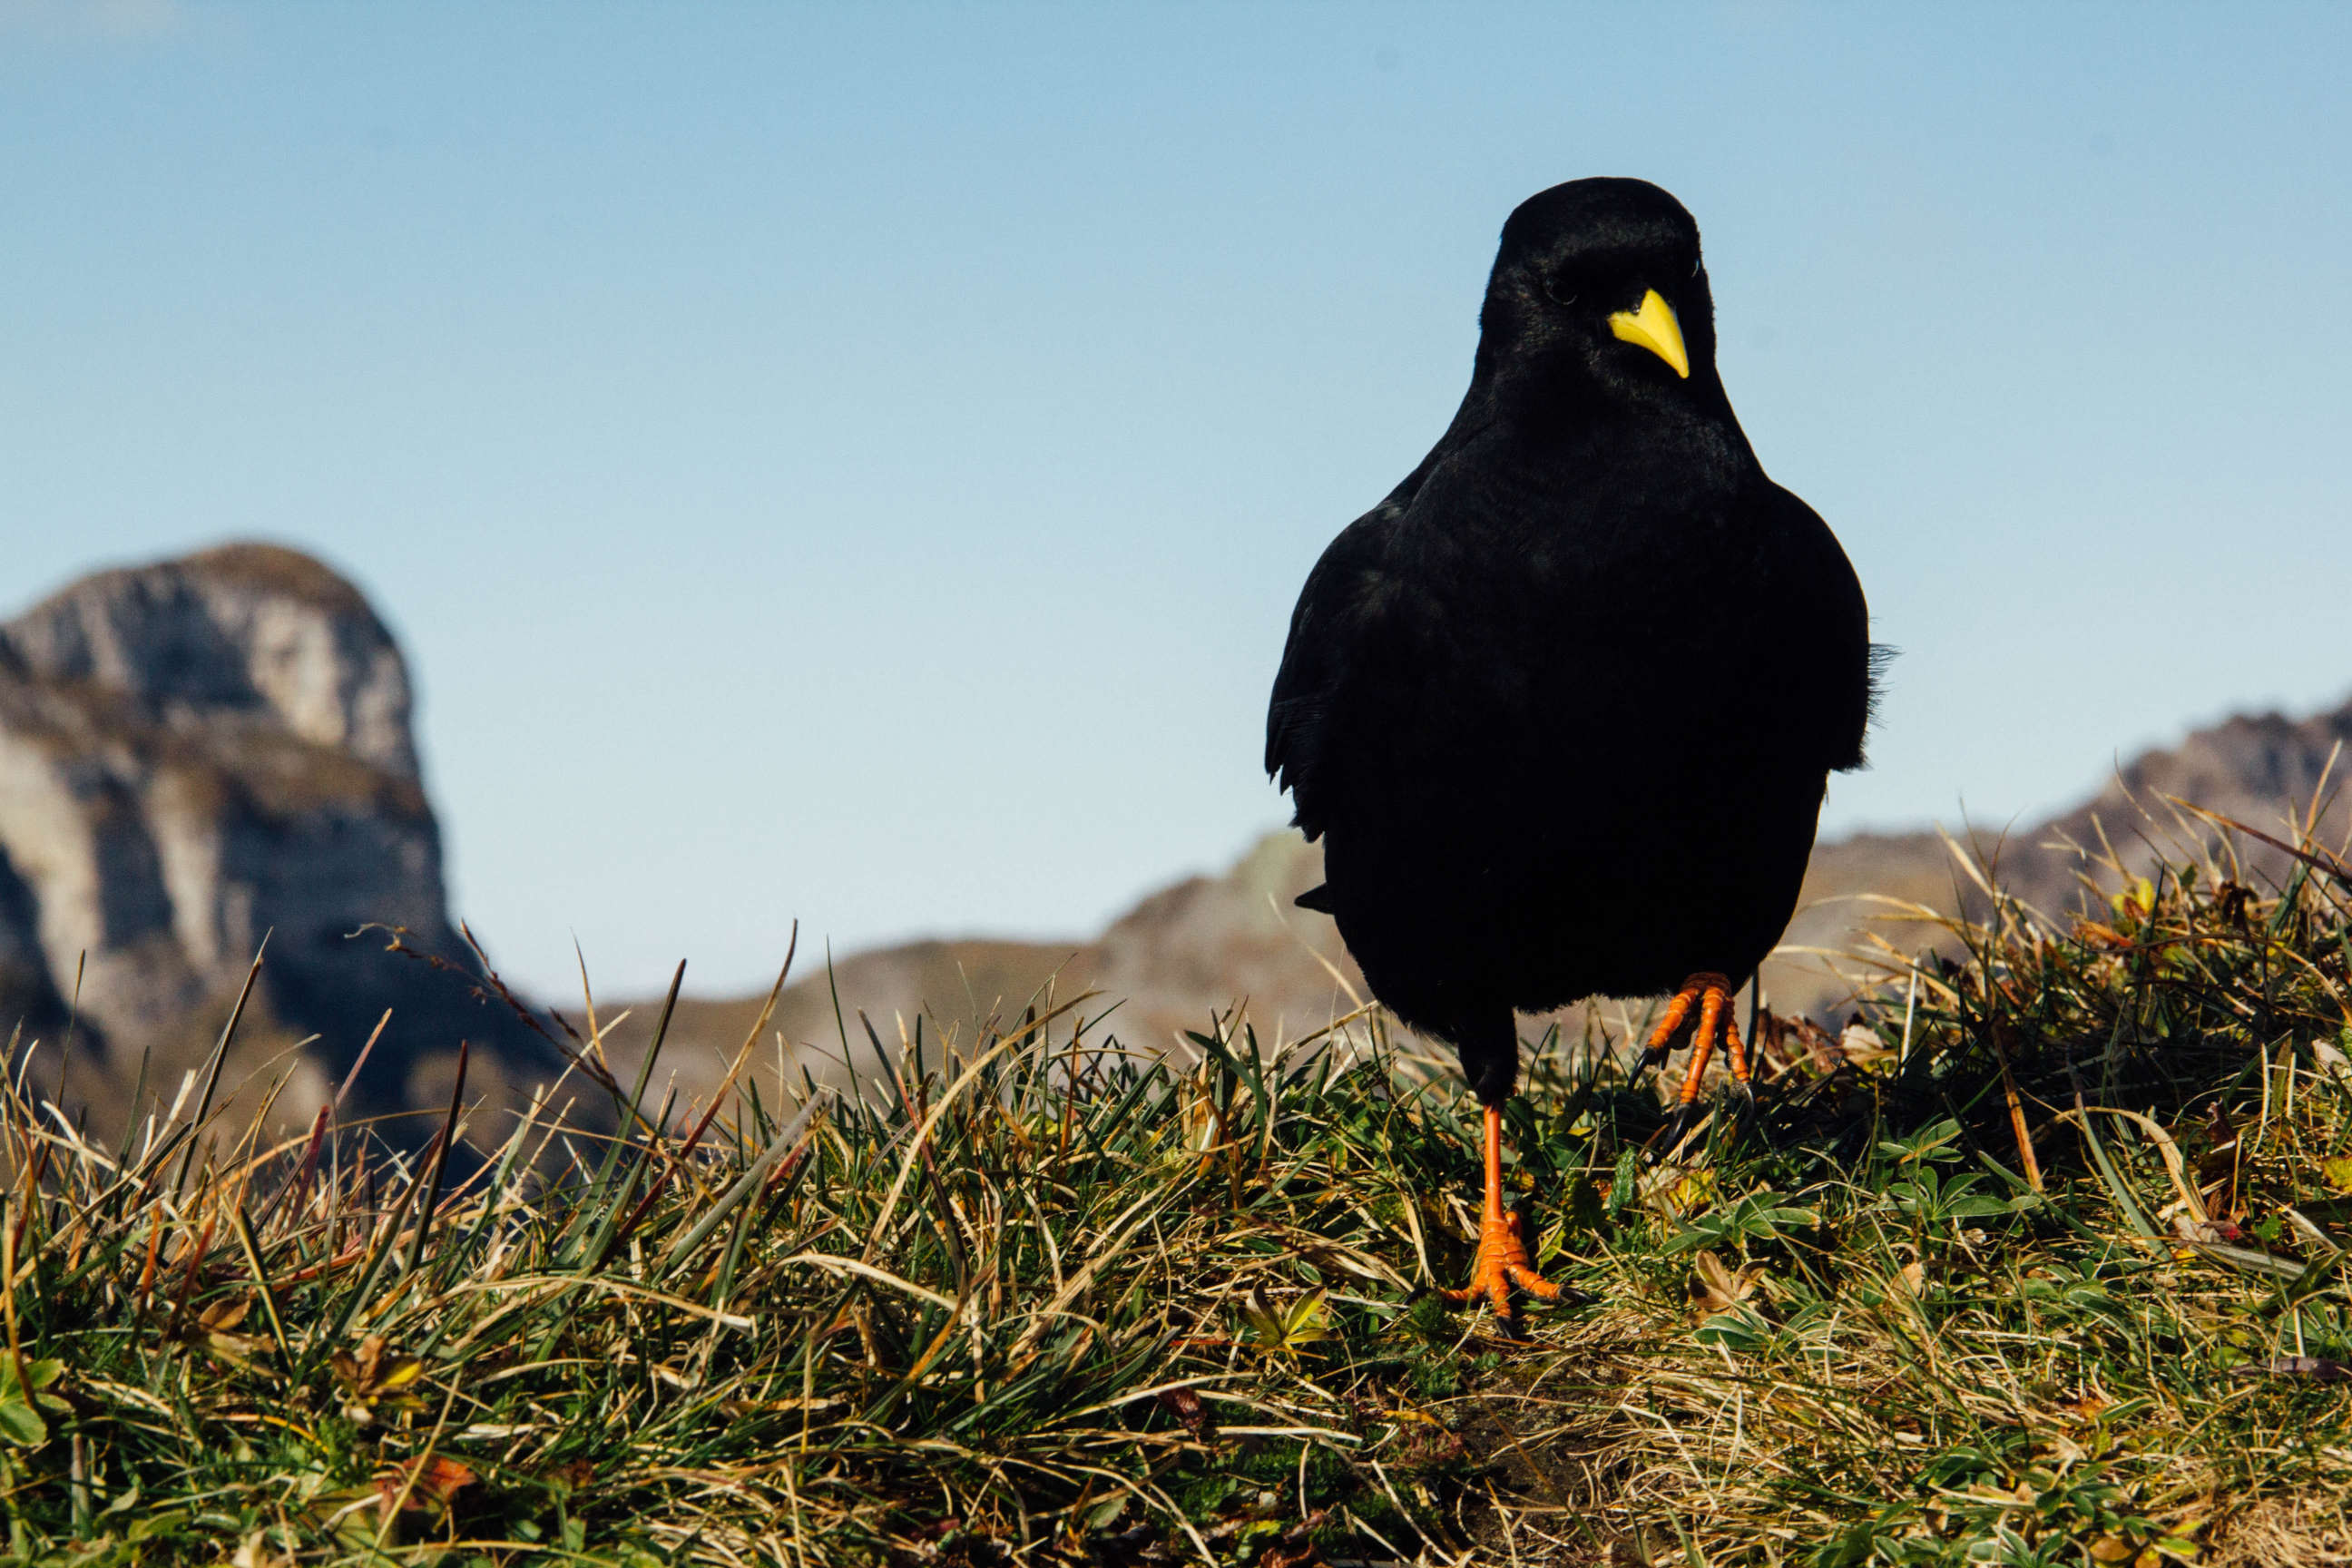
\includegraphics[width=\textwidth]{alpendohle.jpg}
    \note{\textcite[Abs. 1]{diani_black_2016}}
    \label{fig:alpendohle}
\end{figure}

\chapter{Tabelle}
Im folgenden (Tabelle \ref{tab:tabelle}) ist ein Beispiel einer Tabelle:
\begin{table}[ht]
    \caption{Überschrift Tabelle 1}
    \begin{tabularx}{\textwidth} {
        >{\raggedright\arraybackslash}X 
        >{\raggedleft\arraybackslash}X 
        >{\raggedleft\arraybackslash}X}
            \hline
            \multicolumn{3}{c}{\textbf{Beispieltabelle}}\\
            \hline
            \textbf{Linksbündig} & \textbf{Rechtsbündig} & \textbf{Rechtsbündig}\\
            \hline
            Lorem & N/A & N/A\\
            Ipsum & 1 499 & 8 512\\
            Dolor & 297 & N/A\\
            Sit & 1 053 & N/A\\
            \hline
            \textbf{Total} & 2 849 & 8 512\\
            \hline
    \end{tabularx}
    \bigbreak
    \note{Die Beispieltabelle besteht in der ersten Zeile aus einer durchgehenden Zelle mit zentriertem Text. Die restlichen Zellen sind links- oder rechtsbündig.}
    \label{tab:tabelle}
\end{table}

\chapter{Programmcode}
Programmcode ist immer öfter Bestandteil von Studienarbeiten. Die \textcite{American_Psychological_Association_2022} schreibt zur Formatierung von Passagen mit Porgrammcode: "<To present computer code, use a monospace font such as 10-point Lucida Console or 10-point Courier New">. Im Fliesstext könnte dies folgendermassen aussehen: Die Funktion \lstinline{print()} in der Programmiersprache Python wird meist dazu benutzt, Text auf dem Bildschirm auszugeben. Das folgende Beispiel \ref{code:hello} gibt die Zeichenkette "<Hello World"> aus.
\begin{lstlisting}[language=Python,caption=Überschrift Programmcode,label=code:hello] 
# hello_world.py
print("Hello World!")
\end{lstlisting}
\medbreak
\noindent
Weitere Konfigurationsmöglichkeiten für die Darstellung von Programmcode können der Dokumentation\footnote{http://texdoc.net/texmf-dist/doc/latex/listings/listings.pdf} des \texttt{lstlisting} Pakets entnommen werden. 
    % Ende Textteil
    
    % Start Nachspann
    \printbibliography[heading=bibintoc,title={Literaturverzeichnis}]
    \chapterNoNr{Hilfsmittelverzeichnis}


\begin{table}[ht]
\begin{tabularx}{\textwidth}{
    >{\hsize=.3\hsize\raggedright\arraybackslash}X
    >{\raggedright\arraybackslash}X}
        \hline
            \textbf{Hilfsmittel} & \textbf{Prompts}\\
        \hline
        ChatGPT-4, chat.openai.com & a) «Optimiere den Text nach folgenden Kriterien: …» (23.05.23) \newline b) «Generiere eine SPPS-Syntax für…» (24.04.23)\\
        \hline
        DALL-E, labs.openai.com/  & a) «Impressionalist oil painting of a football player» (12.04.23) \\
        \hline
\end{tabularx}
\end{table}
    \appendix
    \chapter{Einseitiges PDF einbinden}
Es ist möglich, PDF als Grafiken einzubinden. Hier ein Beispiel:
\begin{figure}[H]
    \centering
    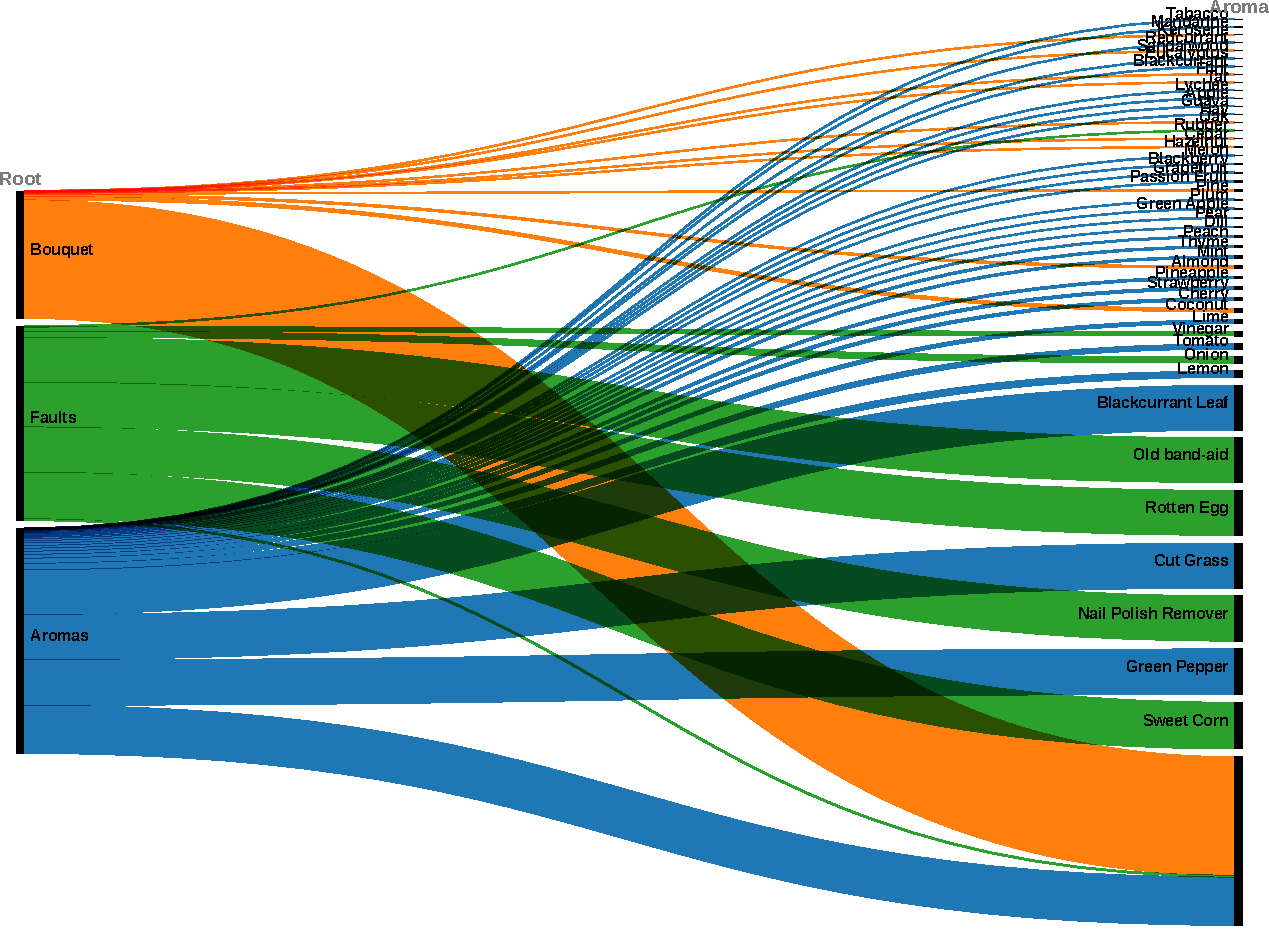
\includegraphics[width=\textwidth]{content/00_assets/example.pdf}
    \caption{Beispiel für Einbindung von PDF-Dateien}
    \label{fig:enter-label}
    \note{Grafik von https://www.rawgraphs.io/}
\end{figure}

\chapter{Mehrseitiges PDF einbinden}
Das Einbinden mehrseitiger PDF ist mittels des \lstinline{pdfpages} Pakets\footnote{https://www.ctan.org/pkg/pdfpages} möglich. Mit dem folgenden Befehl werden die Seiten 9, 15, 25 und 48-50 aus dem books-of-bread PDF eingebunden \parencite{simmons_book_1903}: \\
\lstinline|\includepdf[pages={9,15,25,48-50}]{content/00_assets/book-of-bread.pdf}|

\includepdf[pages={9,15,25,48-50}]{content/00_assets/book-of-bread.pdf}
    \thispagestyle{empty}
\noindent
Ich erkläre hiermit, dass ich diese Arbeit selbstständig verfasst und keine anderen als die angegebenen Quellen und erlaubten Hilfsmittel benutzt habe, einschliesslich der Verwendung von KI-Systemen. Alle Stellen, die wörtlich oder sinngemäss aus Quellen entnommen worden sind, habe ich als solche gekennzeichnet. Ich bin den Vorgaben des Leitfadens wissenschaftliches Arbeiten gefolgt. Mir ist bekannt, dass andernfalls die Hochschulleitung zum Entzug der aufgrund meiner Arbeit verliehenen Qualifikation oder des für meine Arbeit verliehenen Titels berechtigt ist.\\
\\
\\
\\
\ort, \abgabedatum \hfill 
\includegraphics[width=2cm]{content/00_assets/unterschrift.png}\\
Ort, Datum \hfill Unterschrift \autorenschaft

    % Ende Nachspann
    
\end{document}